\chapter{Testen en Resultaten}
\label{chap:testing}

% korte ondubbelzinnige weergave hoe de hardware en software getest is; tests
% per module, integratietest; wat is de testopzet geweest en wat zijn de
% uiteindelijke resultaten; voldoet het aan de gestelde eisen; duidelijk
% omschrijven welke eventuele problemen er nog zijn en hoe deze mogelijk zijn
% te verklaren; eventuele 'work arounds', aanbevelingen; de testen moeten
% zodanig omschreven zijn dat elke test door anderen te reproduceren is

De software en hardware is in verschillende onderdelen getest.
\begin{itemize}
	\item GPIO en servo test;
	\item Camera acquisitie test + benchmark;
	\item Frame processing test.
\end{itemize}

\section{GPIO en servo}
\label{sec:gpioTest}

\subsection{Software}
\label{sub:gpioSoft}
Op basis van een aantal tutorials is er test code geschreven om een GPIO te
testen. Met een multimeter kan er gecontrolleerd worden of de GPIO correct
geconfigureerd is. Daarnaast kan er met een draadje een knopje gesimuleerd
worden.

De GPIO's waren redelijk snel werkend mede dankzij de duidelijke tutorials
beschikbaar voor de BeagleBone Black.

De servo's worden via hardware PWM aangestuurd. Met dank aan wat informatie
op het internet en de GPIO tutorials was de PWM zo aan de praat. Middels een
simpele transistor schakeling is er een servo aan een hardware PWM pin te koppelen.
Door eerst een LED te laten dimmen kan de PWM functie gevalideerd worden.
Vervolgens wordt er een servo aan gekoppelt om de PWM frequentie en puls breedte
te bepalen.

Na de tests is er test software geschreven voor alle hardware aansturingen
zodat er via de command line de interface getest kon worden.

\subsection{Hardware}
\label{sub:gpioHard}

De hardware is eerst op een bench getest om eventuele schade als gevollig van
een foutief ontwerp aan de BeagleBone Black te voorkomen. Alle pinnen zijn
nagemeten voor eventuele kortsluitingen. Daarnaast is de flip-flop schakeling
los van de rest van het systeem getest.

Na een test bleek de flip-flop schakeling niet helemaal te werken. Dit is opgelost
door een RC schakeling tussen de /Q output en D input. Daarna bleken de MOSFETs
ook niet helemaal correct te werken. Het bleek dat de MOSFETs niet voldoende
inschakelen bij 3,3V maar pas vanaf 5V voldoende stroom door laten. Dit probleem
is eenvoudig opgelost middels een 5V pull-up weerstand en een 2,4V zener diode
(zie bijlage \ref{app:sig-conv-schematic} en \ref{app:sig-conv-pcb}).

\section{Camera acquisitie}
\label{sec:camAcq}

De camera acquisitie is geschreven op basis van een tutorial voor video for
linux. Gezien de acquisitie met voldoede snelheid moet gebeuren is er een
benchmark uitgevoerd op de code. Met een frame-rate van 10 - 30fps is er
geconcludeerd dat de acquisitie voldoende snelheid heeft om een prima
systeem te bouwen.

\section{Frame processing}
\label{sec:framePross}

Veel van de operatoren om het frame te verwerken zijn al gemaakt voor het
practicum. Deze zijn dus uitgebreid getest via de QT applicatie en op het
target. Daarnaast is de code voor de BeagleBone Black omgebouwd om een
plaatje in te lezen, het plaatje te verwerken en een plaatje als output
te geven. Dit omdat het systeem van het practicum geen kleuren plaatjes
accepteerd. Op deze manier is het dus wel mogelijk om de RGB filter te
testen.

De resultaten spreken voor zich.

Het originele plaatje is te zien in afbeelding \ref{fig:org}. Vervolgens is deze
gefiltered met een rood-filter (afbeelding \ref{fig:redFilter}). Omdat alle date
goed zichtbaar moet zijn wordt een contrast stretch uitgevoerd (afbeelding \ref{fig:contastStretch})
waarna de afbeelding gethreshold kan worden (afbeelding \ref{fig:threshold}).
Omdat blobs die zich aan de rand van een frame bevinden niet betrouwbaar zijn
moeten deze verwijderd worden (afbeelding \ref{fig:removeBorderBlobs}) en om
eventuele schitteringen of reflecties tegen te gaan worden ook gaten in blobs
gevuld (afbeelding \ref{fig:fillHoles}). Uiteindelijk worden de blobs gelabeled
(afbeelding \ref{fig:labelBlobs}) en geanalyseerd waarna hier uit komt dat
(in de voorbeeld uitbeelding) de zwaarste blob (en dus de marker) zich bevindt
rond coordinaat (322, 325).

\begin{figure}[b]
    \begin{center}
        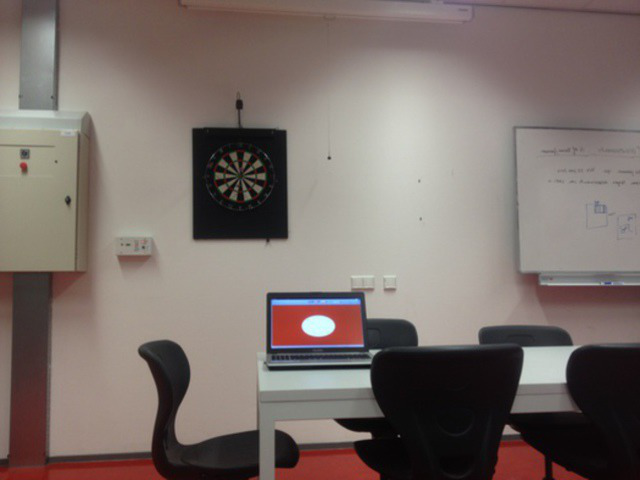
\includegraphics[scale=0.35]{figures/vision/original.png}
    \end{center}
    \caption{Het originele plaatje.}
    \label{fig:org}
\end{figure}

\begin{figure}
    \begin{center}
        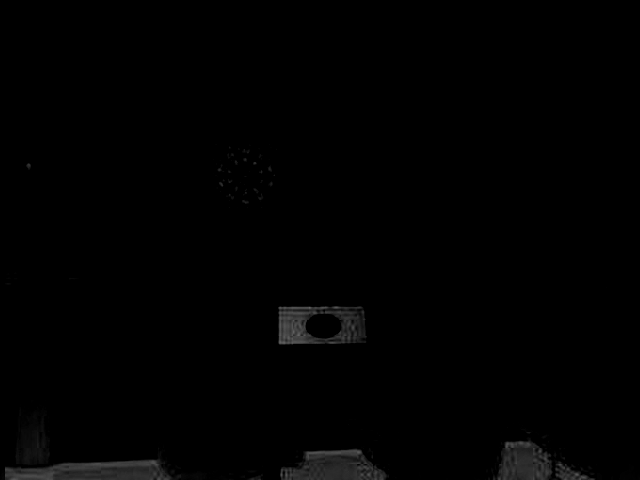
\includegraphics[scale=0.35]{figures/vision/filtered.png}
    \end{center}
    \caption{Het grijswaarde plaatje na de rode filter.}
    \label{fig:redFilter}
\end{figure}

\begin{figure}
    \begin{center}
        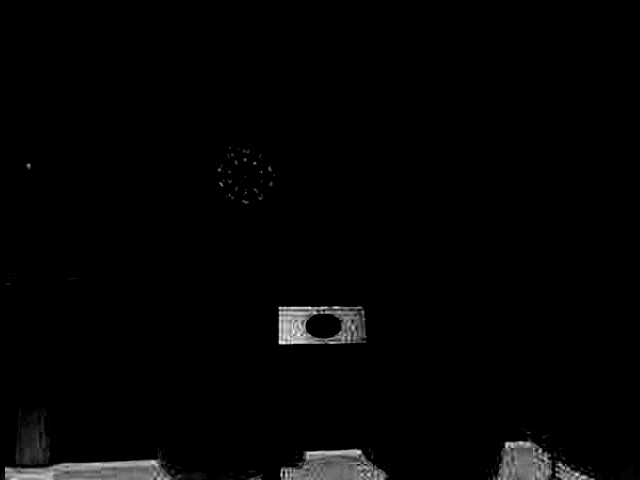
\includegraphics[scale=0.35]{figures/vision/stretched.png}
    \end{center}
    \caption{Het grijswaarde plaatje na de contrast stretch.}
    \label{fig:contastStretch}
\end{figure}

\begin{figure}
    \begin{center}
        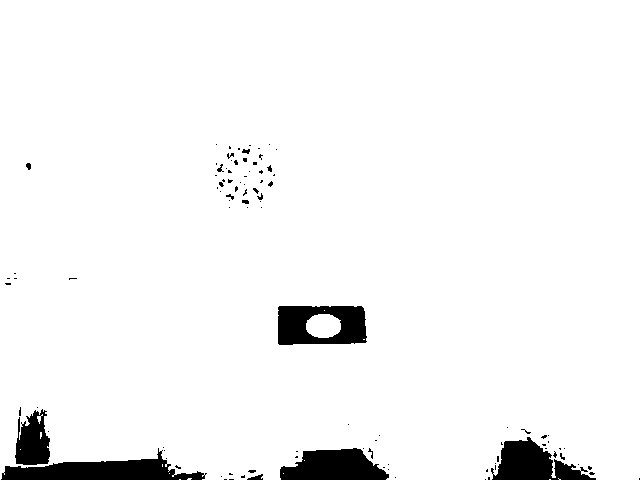
\includegraphics[scale=0.35]{figures/vision/thresholded.png}
    \end{center}
    \caption{Het binaire plaatje na de threshold.}
    \label{fig:threshold}
\end{figure}

\begin{figure}
    \begin{center}
        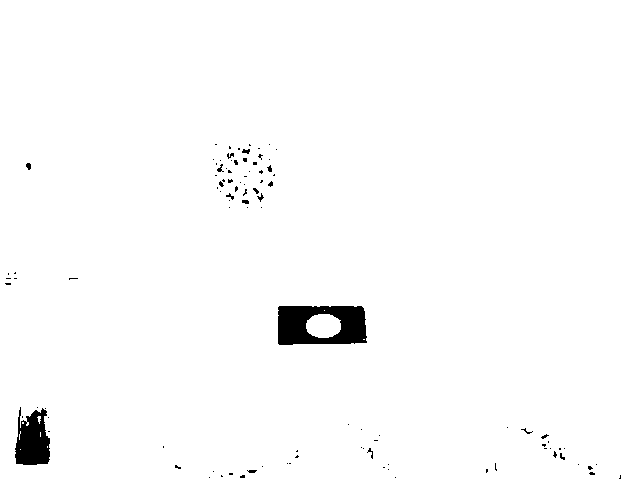
\includegraphics[scale=0.35]{figures/vision/borders.png}
    \end{center}
    \caption{Het binare plaatje na het verwijderen van de blobs aan de randen.}
    \label{fig:removeBorderBlobs}
\end{figure}

\begin{figure}
    \begin{center}
        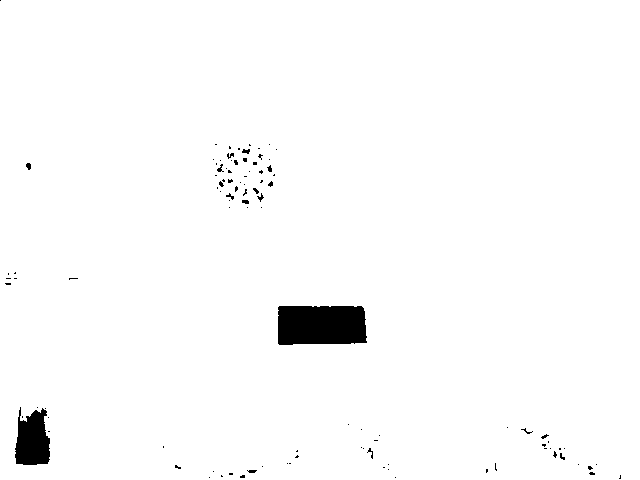
\includegraphics[scale=0.35]{figures/vision/holes.png}
    \end{center}
    \caption{Het binaire plaatje na een \emph{fill holes} operatie.}
    \label{fig:fillHoles}
\end{figure}

\begin{figure}
    \begin{center}
        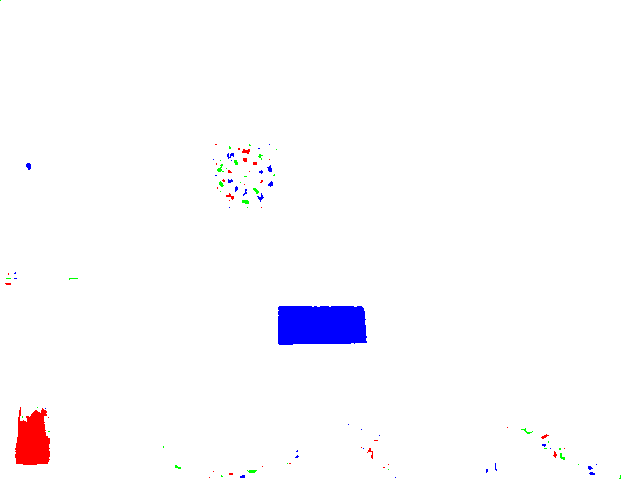
\includegraphics[scale=0.35]{figures/vision/labeled.png}
    \end{center}
    \caption{Het gelabelde plaatje.}
    \label{fig:labelBlobs}
\end{figure}
